\chapter{Структура геометрического решателя}\label{ch:geomsolver}
% Описание главы

Решатель геометрических ограничений представляет собой программное обеспечение (отдельное приложение или программная библиотека), который позволяет создавать задачу геометрических ограничений и соответственно её решать. Основной интерес представляет внутреннее устройство решателя, которое будет рассмотрено в данной главе. Для удобства представления,  решатель можно структурно разделить на три уровня: верхний, средний и нижний. Эти уровни работают последовательно и различными способами преобразуют исходную задачу, что в итоге приводит к её решению. Решение задачи, в зависимости от исхода может быть получено на разных уровнях. Далее будет рассмотрен каждый из представленных уровней.




\section{Верхний уровень}
Данный уровень представляет собой набор модулей, которые работают с представлением задачи в виде набора геометрических объектов и ограничений связывающих их, которые могут быть представлены в виде  мультиграфа, как на рисунке \ref{fig:im1}. Вершинами такого графа являются геометрические объекты, а рёбра соответствуют геометрическим ограничениям заданным между парой объектов (или в случае ограничений действующих на один объект, ребро замыкается на одной вершине). 

\begin{figure}[h]
	\centering
	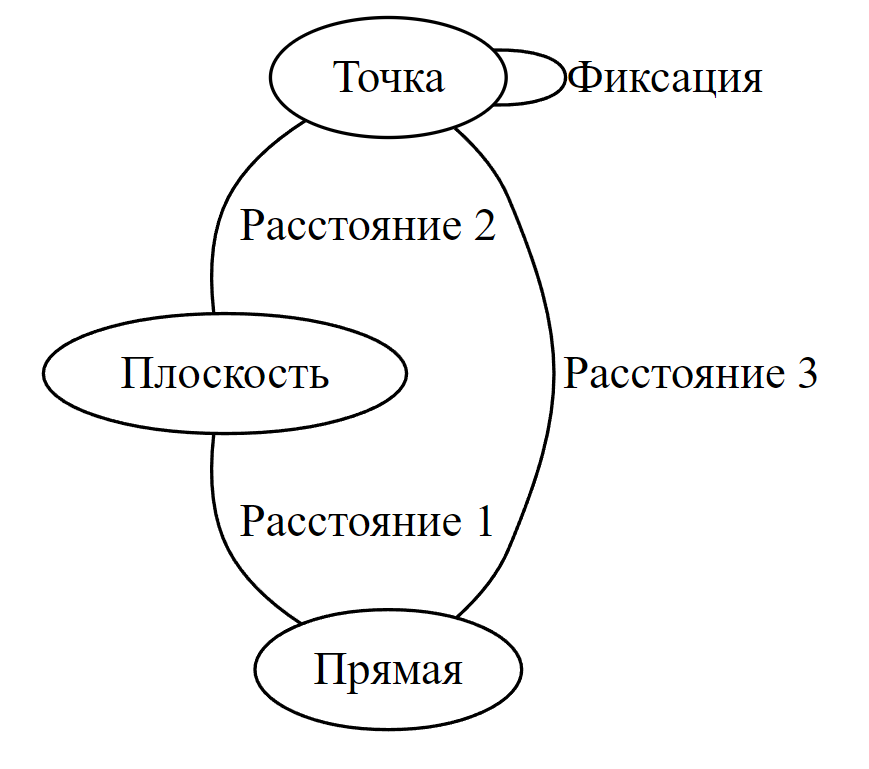
\includegraphics[width=0.5\linewidth]{figures/fig_1_model_graph.png}
	\caption{Пример графа простой геометрической модели}
	\label{fig:im1}%ссылка на картинку
\end{figure}

На данном уровне работает несколько модулей. Важное значение имеет модуль \textit{геометрической декомпозиции}, который способен разделять задачу на подзадачи меньшего размера, что позволяет достичь уменьшения времени решения и увеличения вероятности того, что  решение будет найдено. На этом уровне, также может происходить аналитическое решение небольших задач, исходя из геометрических соображений. Результатом работы этого уровня является одна или несколько подзадач, которые далее требуют непосредственного решения. Также стоит отметить, что на данном этапе возможен исход, при котором исходная задача может и не измениться. Результат работы модуля в виде набора геометрических объектов и ограничений, далее обрабатывается средним уровнем.

Помимо модуля геометрической декомпозиции на данном уровне находится \textit{модуль трансформации}. Его задачей является преобразование сложных ограничений в набор элементарных ограничений. Таким образом, некоторые из поддерживаемых ограничений реализуются в виде набора других более простых ограничений, и отвечает за такое преобразование рассматриваемый модуль. 




\section{Средний уровень}\label{sec:middle_level}
На данном уровне происходит преобразование задачи удовлетворения геометрических решений к алгебраической задаче решения нелинейной системы алгебраических уравнений (далее для краткости СНАУ). Данным преобразованием занимается модуль генерации системы уравнений, который принимает геометрическую модель в виде графа объектов и ограничений, а на выходе предоставляет СНАУ. Помимо данного модуля, к среднему уровню можно отнести так же модули валидации и нормализации. 

\textit{Модуль генерации систем уравнений} является основой среднего уровня. Именно тут происходит основное преобразование задачи удовлетворения геометрических ограничений в задачу решения СНАУ. Данный модуль работает в два этапа. Сначала происходит моделизация геометрических объектов, т.е. описание положения геометрических объектов с помощью набора переменных. Далее для каждого ограничения из задачи генерируется одно или несколько нелинейных, в общем случае, уравнений относительно переменных, с помощью которых описываются геометрические объекты задачи. Подробно устройство данного модуля будет описано в главе \ref{ch:modeler}.

\textit{Модуль нормализации} отвечает за приведение параметров ограничений и объектов к некому каноническому виду, на который опирается модуль генерации уравнений. Параметрами объектов являются их координаты, вектора направлений и для некоторых объектов радиус (или даже радиусы). И например, вектора направлений необходимо нормировать, поскольку все генерируемые уравнения полагаются на единичную длину таких векторов. Не числовыми параметрами ограничений являются такие сущности как выравнивание (т.е. для ограничений в которых направляющие вектора параллельны, этот параметр регулирует направленность этих векторов), ориентация (применима в сосновом для ограничений расстояния и указывает положения объектов относительно нормали одного из них) и др. Также у некоторых ограничений, называемых параметрическими имеются вещественные параметры. К таким ограничениям относят расстояние, угол и радиус. Так же к параметрам ограничений можно отнести такие сущности как вспомогательные точки. Они позволяют конкретизировать точку на поверхности в которой будет удовлетворяться заданное ограничение. Все описанные параметры, в существенном ряде случаев требуют приведения к каноническому виду. Так например, вспомогательные точки обычно перемещаются из заданного пользователем положения в ближайшее положение на поверхности. Или же, например, отрицательное расстояние переводится в положительное и параметр ориентации для расстояние изменяется на противоположенное значение. Данный модуль, отнесён к среднему уровню на основании того, что он не преобразует модуль структурно, т.е. в ходе преобразований не изменяется число и тип объектов, а также не изменяются аргументы ограничений, в отличии от модуля геометрической декомпозиции. Также данный модуль обладает "знанием" о каноническом виде ограничений и объектов, на которое полагается модуль генерации уравнений. 

Ещё одним модулем среднего уровня является \textit{модуль валидации}. Данный модуль отвечает за проверку ограничений из модели на удовлетворенность. Таким образом результатом работы модуля является статус (в простейшем случае двузначного тип) о удовлетворенности всех ограничений. Помимо статуса, модуль выдаёт также численную меру удовлетворенности ограничений. Причём в данную меру входят два параметра: угловая и линейная погрешности. Угловая погрешность вычисляется для векторов направлений, а линейная вычисляется для координат объектов. Тем самым данный модуль, используется в двух случаях. Во-первых для проверки корректности численного решения (т.е. дополнительная проверка помимо невязки самих уравнений), что позволяет легче обнаруживать ошибки в модуле генерации уравнений так и в модуле решения СНАУ. Во-вторых, этот модуль требуется в самом начале работы геометрического решателя, чтобы избежать дальнейшей работы, в случае если пользователь задал изначально удовлетворённую модель. Этот модуль отнесён к среднему уровню, поскольку он в значительной степени согласован с модулем генерации уравнений, т.к. погрешности для ограничений вычисляются подобно вычислению невязки в уравнениях, описывающих данное ограничение.




\section{Нижний уровень} \label{sec:low_level}
Данный уровень ответственен за решение СНАУ, которая генерируется на среднем уровне. Представителями этого уровня являются модули решения системы нелинейных уравнений и алгебраической декомпозиции. 

\textit{Модуль решения СНАУ} реализует итеративный алгоритм Ньютона - Рафсона. Выбор этого метода обусловлен тем, что он способен решать как переопределенные, так и недоопределенные системы нелинейных уравнений \textbf{[тут нужна ссылка на источник подтверждающий мои слова]} и хорошо-определенные системы тоже. Данный алгоритм требует вычисления якобиана системы на на каждой итерации. В некоторых модификациях якобиан обновляется лишь через несколько итераций. Помимо этого, на каждой итерации решается СЛАУ, матрицей которой как раз и является якобиан системы. Эта операция является самой дорогой в терминах вычислительной сложности, поэтому сложность решения СНАУ оценивается как \cite{GoluVanl96}:
\begin{equation*}
    O(L \cdot m \cdot n^2)
\end{equation*}
если $m > n$, иначе:
\begin{equation*}
    O(L \cdot n \cdot m^2)
\end{equation*}
где $n$ -- число переменных, $m$ -- число уравнений, $L$ -- число итераций метода Ньютона. Число итераций метода в общем случае неизвестно, т.к. он не гарантирует сходимости с произвольной начальной точки. Поэтому оно ограничивается сверху эмпирически подбираемым значением, которое в худшем случае не будет приводить к существенным задержкам, когда метод не сходится. Помимо ограничения сверху, могут быть использованы различные эвристики, для преждевременной остановки решения. Например, если несколько итераций подряд норма шага метода близка к нулю, то можно прекратить решение. \textbf{/* Здесь также можно написать про ещё одну эвристику с рекордом на N прошлых итерациях*/}

\textit{Модуль алгебраической декомпозиции} производит разбиение, другими словами декомпозицию, системы уравнений на несколько подсистем, которые далее решаются по отдельности, в заданном порядке. В основе работы модуля лежит алгоритм декомпозиции двудольных графов Далмейджа-Мендельсона \cite{dulmage1958coverings}. Алгоритмическая сложность такой декомпозиции меньше чем сложность алгоритма решения СНАУ. таким образом этот модуль позволяет в ряде случаев достичь ускорения при решении, по сравнению с решением системы уравнений целиком. Для своей работы, данный алгоритм требует поиска переменных, от которых зависит каждое их уравнений системы. Это требуется для построения двудольного графа зависимостей для системы уравнений. Далее, алгоритм предоставляет набор подсистем, которые необходимо решить в заданном алгоритмом порядке. Более детально рассматриваемый модуль будет описан в одной из следующих секций.
